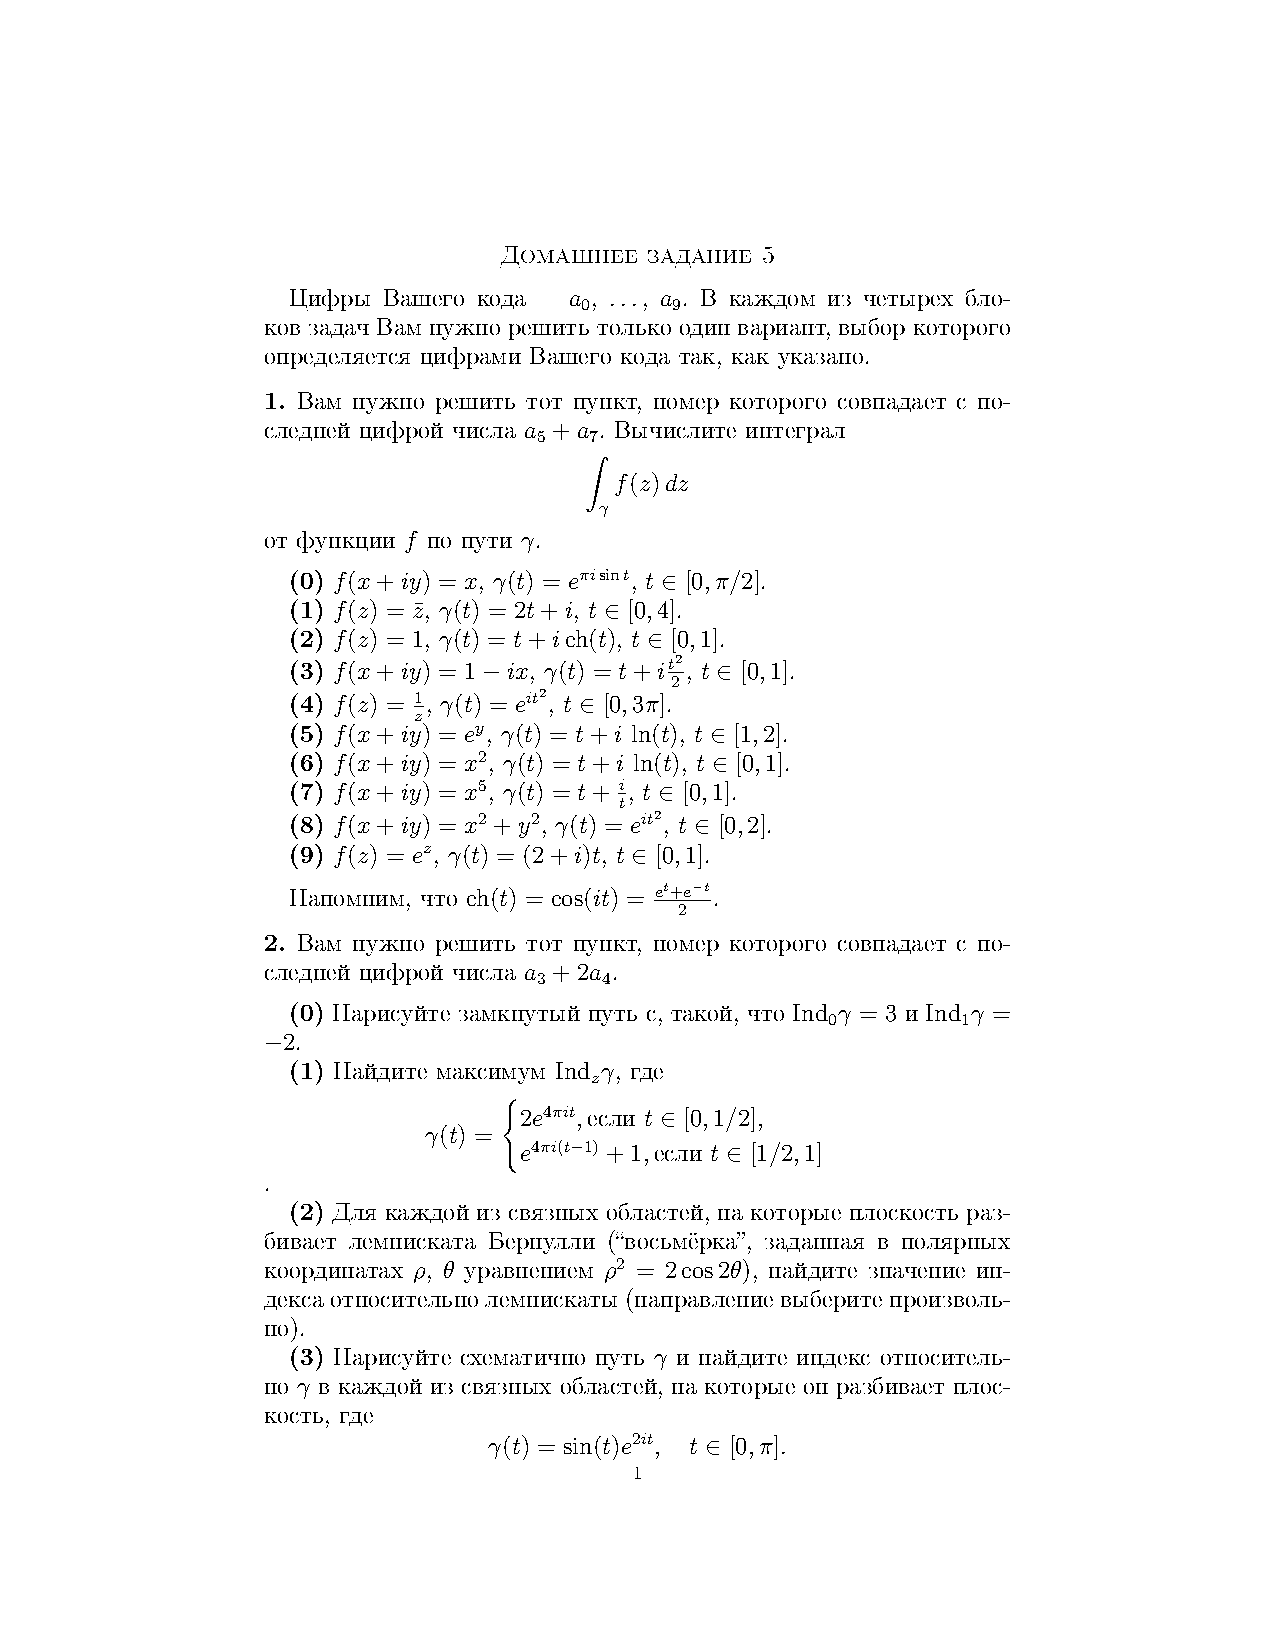
\includepdf[scale=1,pages=1-4]{Tasks/hw5}
\newpage
\section*{Решения}
\subsection*{Задача 1}
	Необходимо решить задачу $a_5 + a_7 = 6 + 3 = 9 \mod 10$
	\begin{gather*}
		f(z) = e^z,\ \gamma(t) = (2 + i)t,\ t \in [0,1]\\
		\int_{\gamma}f(z)dz 
		= \int_{0}^{2+i} f((2+i)t) \cdot (2+i) dt\\
		= \int_{0}^{2+i} e^{(2+i)t} \cdot (2+i) dt
		= (2+i) \int_{0}^{2+i} e^{(2+i)t}dt
		= \int_{0}^{(2+i)^2} e^{(2+i)t}dt\\
		= e^{(2+i)^2} - e^0
		= e^{(2+i)^2} - 1
		= e^{3 + 4i} - 1
	\end{gather*}
\vskip 0.4in

\subsection*{Задача 2}
	Необходимо решить задачу $a_3 + 2a_4 = 9 + 2 \cdot 7 = 3 \mod 10$
	\begin{gather*}
		\gamma(t) = \sin(t)e^{2it},\ t \in [0, \pi]
	\end{gather*}
	\begin{figure}[h]
		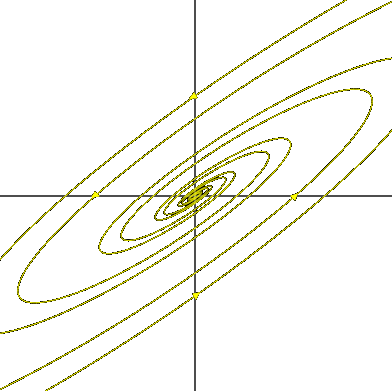
\includegraphics[width=0.5\linewidth]{Pic5}
	\end{figure}
	Данная функция задает кардиоиду, индекс внутри нее равен 1, снаружи 0.
\vskip 0.4in

\subsection*{Задача 3}
	Необходимо решить задачу $5a_0 + 7a_1 = 5 \cdot 1 + 7 \cdot 7 = 4 \mod 10$
	Контур не проходит через $0,i,-i$
	\begin{gather*}
		\frac{2}{z^3 + z} = \frac{2}{z} - \frac{2z}{z^2+1} = \frac{2}{z} - \frac{1}{z + i} - \frac{1}{z - i}
	\end{gather*}
	и $\int_{\gamma \circ \varphi} f(z)dz = \int_{\gamma} f(z)dz$, если $\varphi$ -- биекция. Так как $C$ не имеет самопересечений, то он биективен окружности, то есть $\int_{C} f(z)dz = \int_{\gamma} f(z)dz$ и $\operatorname{Ind}_a \gamma = 0$ или $1$.
	\begin{gather*}
		\gamma: [0,2\pi] \to \mathbb{C}\\
		\int_{\gamma} f(z)dz = \int_{0}^{2\pi} f(\gamma(\theta)) \gamma'(\theta) d\theta\\
		\gamma(\theta) = r e^{i \varphi}\\
		f(z) = \frac{2}{z}\qquad f(\gamma(\theta)) = \frac{1}{re^{i \varphi}}\\
		\int_{\gamma} \frac{2}{z}
		= 2\int_{0}^{2\pi} \frac{\gamma'(\theta)}{f(\gamma(\theta))} d\theta
		= 2\int_{0}^{2\pi} \frac{ire^{i \varphi}}{r e^{i \varphi}} d \theta
		= 2\int_{0}^{2\pi} i d\theta = 4\pi i
	\end{gather*}
	Аналогично $-\int_{\gamma} \frac{dz}{z + i} = -	2\pi i$ и $-\int_{\gamma} \frac{dz}{z - i} = -	2\pi i$, откуда
	\begin{gather*}
		\int_{C} f(z)dz = 2\pi i k_1 - 2 \pi i k_2 - 2\pi i k_2
	\end{gather*}
	Где $k_i = 0,1$ -- индекс точки
\vskip 0.4in

\subsection*{Задача 4}
	Необходимо решить задачу $6a_1 + a_6 = 6 \cdot 7 + 9 = 1 \mod 10$
	\begin{gather*}
		\int_C f(z)dz = 1,\quad \int_{C}zf(z)dz = -1
	\end{gather*}
\vskip 0.4in
